\documentclass[12pt, titlepage]{article}

\usepackage{cite}
\usepackage{graphicx} 
\usepackage{fullpage}
\usepackage{subcaption}
\usepackage{wrapfig}
\usepackage{float}
\usepackage{pdfpages}

% Alter some LaTeX defaults for better treatment of figures:
    % See p.105 of "TeX Unbound" for suggested values.
    % See pp. 199-200 of Lamport's "LaTeX" book for details.
    %   General parameters, for ALL pages:
    \renewcommand{\topfraction}{0.9}	% max fraction of floats at top
    \renewcommand{\bottomfraction}{0.8}	% max fraction of floats at bottom
    %   Parameters for TEXT pages (not float pages):
    \setcounter{topnumber}{3}
    \setcounter{bottomnumber}{3}
    \setcounter{totalnumber}{4}     % 2 may work better
    \setcounter{dbltopnumber}{2}    % for 2-column pages
    \renewcommand{\dbltopfraction}{0.9}	% fit big float above 2-col. text
    \renewcommand{\textfraction}{0.07}	% allow minimal text w. figs
    %   Parameters for FLOAT pages (not text pages):
    \renewcommand{\floatpagefraction}{0.7}	% require fuller float pages
	% N.B.: floatpagefraction MUST be less than topfraction !!
    \renewcommand{\dblfloatpagefraction}{0.7}	% require fuller float pages

\title{Link Signature Keying for Skeptics}
\author{{\normalsize K.~C.~Kerby-Patel}}
\date{}

\begin{document}
\bibliographystyle{ieeetran}
\begin{titlepage}
\maketitle
\end{titlepage}
\section*{Project Summary}
\thispagestyle{empty}

\subsection*{Intellectual Merit}
This work represents a new paradigm for analysis of link signature based security techniques, grounded in the physics of the propagation channel.  It identifies and addresses a major gap in the present understanding of issues surrounding practical implementation and adoption of LSK by applying estimation theoretic concepts to model the capabilities of a sophisticated eavesdropper.  Ultimately, the proposed approach will strengthen the security of LS based security strategies, allowing identification of suitable channels for LSK, development of defensive strategies for legitimate nodes, and evaluation of information theoretic security metrics for LSK scenarios.

\subsection*{Broader Impacts}
%"Some examples are: designing innovative courses or curricula; conducting outreach and mentoring activities to enhance scientific literacy or involve students from groups that have been traditionally underrepresented in science; researching students' learning and conceptual development in the discipline; incorporating research activities into undergraduate courses; linking education activities to industrial, international, or cross-disciplinary work; and implementing innovative methods for evaluation and assessment."

%The proposed project depends on understanding 
	%wave behavior
	%phase
	%superposition
%as well as
	%probability/statistics/random processes
	%information theory
	%particularly data processing inequality and mutual info
	%estimation theory

%outreach activities - early introduction of wave concepts?
	%if at UMB, develop an ``innovative'' course in communication theory with emphasis on wireless channel and its behavior, plus statistics - perhaps with some kind of outreach thing like an encryption wars
%improving representation of women/underrepresented groups in engineering/mentoring/etc.
	%if at NEU, support a co-op or something where they can work on this?
	%if I do something like this, how related does it need to be to the research topic?
\newpage
\setcounter{page}{1}
\section*{Objectives}
%big problem
Modern life depends on encryption to protect sensitive information.  At present, encryption keys are shared either via computational key exchange methods like Diffie-Hellman, or by the physical distribution of security tokens.  Both these methods have disadvantages: computational key exchange is potentially vulnerable to quantum computing, while physical key management and distribution is logistically difficult and expensive.  Link signature keying (LSK) has been proposed as an alternative to both methods.  

%ref to lit #1
LSK is a promising new approach to encryption which uses the inherent reciprocity and location dependence of the wireless channel to generate a random number seed for symmetric key generation \cite{hershey1995, hassan1996, azimisadjadi2007, mathur2008}.  It has applications as an alternative to physical key management because nodes can generate symmetric keys without a physical meeting.  It is also interesting as an alternative to computational key exchange because it has been claimed to be information theoretically secure and would therefore not be vulnerable to quantum computing \cite{ye2010}.  
%needs a figure here to show how LSK works - maybe RSS -> bits?

%ref to lit #2
However, many security claims related to LSK rest on na\"{i}ve assumptions about the probabilistic behavior of wireless channels.  Research on LSK has largely ignored the underlying physical behavior of the wireless channel, which results in optimistic conclusions about its security.  In particular, since LSK depends on the physical behavior of the wireless channel, the security metric of LSK is typically stated as a minimum secure distance (MSD) beyond which an eavesdropper would be unable to estimate the channel transfer function and derive the legitimate nodes' key. 

Current practice is to use the channel correlation length as the MSD.  However, this usage discounts the fact that channel observations are a deterministic function of slowly-varying environmental parameters which can persist over distances much greater than the correlation length \cite{jakes1974, duel-hallen2007}.  It has been pointed out in \cite{he2013} that many practical channels have correlation lengths longer than a wavelength (which is commonly assumed to be an appropriate MSD); this work goes further to argue that correlation length in general is not applicable to LSK, even in channels with short correlation lengths.  Our initial work has indicated that a more conservative MSD is needed, since
%the correlation-based understanding of the MSD is indeed inappropriate, and 
a sophisticated eavesdropper could predict the channel at distances much greater than the correlation length \cite{kckpVTC2015, brown2015}.  


%this is the part with the hero narrative
The objective of this proposal is to produce a more conservative, robust, and trustworthy understanding of LSK security informed by the physics of the propagation environment.  We propose an alternative paradigm, based on information theory and estimation theory and grounded in physical wave propagation behavior.  An LSK eavesdropper's channel prediction problem has parallels in remote sensing topics like direction of arrival estimation, which makes LSK well suited to an electromagnetics-based approach despite its superficial connection to cryptography.

The proposed framework will ultimately provide
%
a definitive answer on the question of LSK's information theoretic security 
%
and a more conservative means to estimate the MSD.  It will also 
%
permit the analysis of more sophisticated eavesdropper geometries and 
%
defensive strategies for legitimate nodes.  Collectively, these objectives 
%
move toward establishing the viability of LSK as a practical encryption method and as an alternative to physical key management and computational key exchange schemes.

\section*{Research Plan}
\subsection*{Background}
Link signature keying schemes have been proposed by a number of authors in recent years.  All implementations of LSK rely upon two particular qualities of the wireless propagation channel: first, that it is reciprocal, since the channel transfer function between a pair of locations is the same when measured in both directions; and second, that in a sufficiently scattering-rich environment it is strongly location-dependent. 
%would like to put specific refs that use each technique next to the technique (phase vs. RSS, privacy amp, key reconciliation)

\begin{wrapfigure}{r}{0.5\textwidth}
\begin{center}
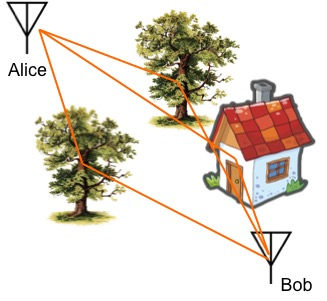
\includegraphics[width=0.4\textwidth]{BasicScenario}
\caption{Notional link signature keying scenario with legitimate nodes Alice and Bob.}\label{scenario}
\end{center}
\end{wrapfigure}
In a typical LSK implementation (Figure \ref{scenario}), legitimate nodes Alice and Bob negotiate a key based on their measurements of the wireless channel.  First, Alice transmits a known training sequence or channel sounding waveform, which travels through the propagation environment and interacts with any scatterers that are present.  Bob's observation of the waveform consists of the superposition of many delayed copies of the training sequence after it travels along multiple scattering paths with different delay times and amplitudes. Next, Bob transmits the same training sequence.  Alice also records a version of the training sequence that has been modified by the propagation channel.  Alice and Bob then use their observations and the known training sequence to estimate the channel transfer function, ideally obtaining the same result due to reciprocity.  Depending on the particular scheme, the phase \cite{hershey1995, hassan1996, sayeed2008} or amplitude \cite{azimisadjadi2007, mathur2008, ye2010, premnath2013, jana2013} of the channel transfer function is then quantized.  Alice and Bob may perform information reconciliation and privacy amplification operations on the resulting samples in order to agree on the final key bits.  Finally, Alice and Bob arrive at a shared encryption key.  New key bits may be obtained whenever the environment has changed enough to provide a new channel realization; for mobile terminals this may occur on a time scale of milliseconds \cite{hershey1995}.
 
Because of the location dependence of the channel, it is frequently stated that LSK is secure as long as no eavesdroppers exist within half a carrier wavelength of the legitimate nodes, which corresponds to the correlation length of a Rayleigh fading channel.  He et al. have pointed out that some channels have much longer correlation lengths, and the assumption that the minimum secure distance (MSD) is a half wavelength is often inappropriately optimistic \cite{he2013}.  
It is also observed in \cite{jakes1974} %section 1.6
 that, while mobile terminals may observe short correlation lengths due to large angular spread and nearby scatterers, base stations tend to observe much longer correlation lengths.
 %... because the angular spread is smaller when viewed from that endpoint and the distance to scatterers is larger
These works begin to address the issue of simplistic assumptions about the predictability of channel transfer functions. 
However, it should be noted that \cite{he2013} still supports the use of the channel correlation length as the MSD, with the caveat that in general the correlation length may not be a half wavelength.  In the next section, we will argue that the correlation length is not an appropriate estimator of the MSD in these situations, because it confuses how fading is \emph{modeled} with how it \emph{physically occurs}.  As a result, it produces optimistic security claims by representing a best-case scenario.

\subsection*{Initial Results}
The use of the correlation length as the MSD stems from the application of statistical channel models for communications to LSK scenarios. Most channel models are built on a representation of the channel as a superposition of many scattering paths and potentially a direct path from transmitter to receiver. In narrowband channels, this takes the form of a sum of sinusoids, with random amplitudes and phases selected from a probability distribution representing the aggregate physical properties of scatterers. 
%In general, the model is intended to predict the typical behavior of a system in an ensemble of similar channels, so these parameters are selected from a probability distribution.  

Since most communications applications fundamentally are interested in received power and related quantities like signal to noise ratio, channel models have largely focused on second-order statistics such as the correlation function.  Additionally, many analyses invoke the law of large numbers by assuming there are sufficiently many scatterers that the statistics are approximately Gaussian, which implies that only second-order statistics exist.  If correlation-based eavesdropping approaches were the only possible attacks on LSK systems, second-order statistics would be sufficient to characterize them as well.  However, the LSK eavesdropper problem bears strong similarities to direction of arrival and synthetic aperture radar problems, for which non-correlation approaches already exist.  Thus, a complete security analysis of LSK must be robust enough to address these sophisticated eavesdropper strategies, which incorporate the known physical behavior of multipath scattering.  


%show that use of corr len implicitly uses corr func as proxy for MI and thus assumes Gaussian statistics, which are a lower bound on MI in general\cite{cover2006-jgvars}
The metric of information theoretic security, and in general of an eavesdropper's ability to estimate the legitimate nodes' channel, is the mutual information between the eavesdropper's channel observations $h_{AE}+n_E$ and the legitimate nodes' channel observations $h_{AB}+n_B$ (both in noise). The use of the correlation length as the MSD implicitly uses the correlation function as a proxy for the mutual information function.  If the two channel transfer functions are jointly Gaussian random variables as is usually assumed, the mutual information $I$ is a monotonic function of the statistical correlation $\rho$ \cite{cover2006-jgvars}:
\begin{equation}\label{JGMI}
I(h_{AE}+n_E;h_{AB}+n_B) = -\frac{1}{2}\log (1-\rho^2)
\end{equation}
However, if the channel observations are not jointly Gaussian, (\ref{JGMI}) is merely a lower bound for the mutual information.  In general, channel parameters have been observed to persist longer than the correlation length \cite{jakes1974, duel-hallen2007}.  This indicates that in realistic channels the mutual information may also persist over distances greater than the correlation length, and in this case the mutual information is indeed greater than that indicated by (\ref{JGMI}).


%argue against use of correlation length as proxy for MI because chan params vary so slowly even for quickly varying channels - \cite{jakes1974, duel-hallen2007}
Physically, the channel is a deterministic function of environmental parameters $\vec{\theta}$ that describe nearby scatterers - for instance, the scatterers' positions and the amplitudes and phases of the scattering paths.  These environmental parameters at an arbitrary pair of observer positions have a position-dependent joint probability density function.  The parameters must approach equality (complete dependence) when the distance between observation points approaches zero so that two co-located observers see the same channel, and they must approach complete independence when the distance approaches infinity.
%implicitly, chan params are a random process (function of observer position rather than t, assuming channel is not time-varying)
Then, the mutual information between Eve's and Bob's channel transfer functions $h_{AE}$ and $h_{AB}$ is trivially bounded by $I(\vec{\theta}_{AE};\vec{\theta}_{AB})$ via the data processing inequality; in the case of zero separation between observation points this reduces to the entropy of $\vec{\theta}$.
%madiseh2008 knows about the upper bound based on the data processing inequality but doesn't make the next step to disqualifying the correlation function.

Since the channel parameters do persist over relatively large distances, it is reasonable to assume that only one realization of the random channel parameters exists within an appropriately sized observation window.   In this case, since the parameters are constant within the window, it would be possible to estimate them and predict the channel transfer function.  Spatial prediction of the LSK channel environment was pursued based on its mathematical similarity to temporal channel prediction, which has been demonstrated over extended distances \cite{eyceoz1999, andersen1999, duel-hallen2000, isukapalli2006}.  Temporal channel prediction uses multiple samples of the mobile channel over time to predict future values of the channel transfer function.  Spatial channel prediction similarly uses multiple spatial samples of the channel to predict the channel transfer function at a distance.  Spatial channel prediction for LSK eavesdropping has strong similarities to other well-known estimation problems, including direction of arrival estimation, multilateration, and synthetic aperture radar, depending on the geometry of the eavesdropper's spatial sampling.

\begin{wrapfigure}{l}{0.5\textwidth}
\begin{center}
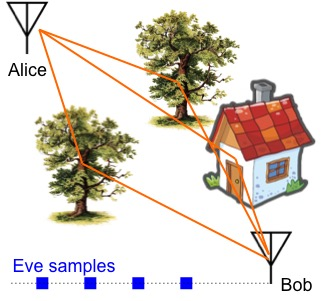
\includegraphics[width=0.4\textwidth]{scenarioEve}
\caption{Modified link signature keying scenario in which Eve can take samples along a line toward one of the legitimate nodes (Bob).}\label{scenarioWithEve}
\end{center}
\end{wrapfigure}
Our approach to this this problem assumes a more sophisticated eavesdropper that may take samples of the channel transfer function at multiple locations, rather than just one.  Initial work has focused on an eavesdropper that takes samples along a line toward one of the legitimate nodes, as shown in Figure \ref{scenarioWithEve}.  

In \cite{kckpVTC2015}, an expression was presented for the Cram\`er-Rao lower bound (CRLB) on an eavesdropper's estimate of the legitimate channel if the eavesdropper is configured as in Figure \ref{scenarioWithEve} and all scatterers are in the far field of the observation window.  The far field restriction on scatterers allows this to be considered as a spectral estimation problem.  Under these circumstances, calculations indicated that an eavesdropper taking multiple spatial samples could estimate the legitimate channel transfer function with very low error at distances greater than a half wavelength, even in channels with wide angular spread.  Figure \ref{CRLB_vs_measLength} shows a plot of the CRLB vs. the length of the eavesdropper's sampling array in a sample channel scenario.  For a given distance at which the legitimate channel transfer function is to be estimated, there exists a critical sampling array length above which the CRLB on the eavesdropper's channel estimate quickly becomes quite small.  This is the case even for prediction distances much larger than the correlation length of the channel.
\begin{figure}
\begin{center}
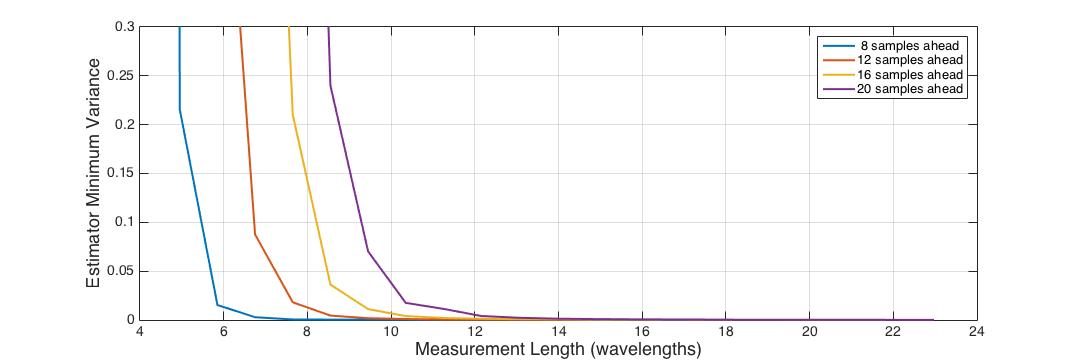
\includegraphics[width=\textwidth]{CRLB_vs_measLen}
\caption{CRLB on eavesdropper's estimate of channel transfer function at a distance of 8, 12, 16, or 20 samples (approx. 4, 6, 8, or 10 wavelengths) vs. length of sampling array in wavelengths for an example scenario with 7 scatterers with uniform probability distribution in angle, SNR = 23 dB, sample spacing = $0.45 \lambda$, and equal scattering path amplitudes.}\label{CRLB_vs_measLength}
\end{center}
\end{figure}
%if space permits, can also include plots of CRLB vs. SNR and other useful metrics.

Subsequent work examined this estimation problem in a simulated channel \cite{brown2015}.  The eavesdropper implementation used MATLAB's built-in rootMUSIC function to estimate the spatial frequency of each scattering path, then applied those results to find the complex amplitude of each scattering path.  The channel transfer function at locations beyond the sampling array was estimated by reconstructing the channel from these parameters assuming a sum-of-sinusoids channel model, which is appropriate as long as all scatterers are in the far field of the observation region.  The simple eavesdropper implementation was tested in a Monte Carlo simulation, with a new randomly generated channel realization in each trial.  

Some results of this simulation are shown in Figures \ref{sim_vs_samples}-\ref{sim_vs_SNR}.  In each trial, the maximum prediction length is defined as the number of samples beyond the sampling array for which the eavesdropper can estimate the channel transfer function with less than 5\% error.  The average maximum prediction length (AMPL) shown in these plots denotes the average of the maximum prediction length over all Monte Carlo trials with the same parameter values.  The figures illustrate the dependence of eavesdropper prediction capability on the scenario parameters: Figure \ref{sim_vs_samples} shows that the eavesdropper has better prediction capability as its sampling length increases; Figure \ref{sim_vs_numScat} shows that the channel prediction problem is more difficult in channels with more scattering paths; and Figure \ref{sim_vs_SNR} shows that the eavesdropper's prediction capability increases with increased signal-to-noise ratio.  In general, the simulation results support the conclusion that in some cases an eavesdropper can estimate the value of the channel transfer function at larger distances than is typically assumed.  It should be pointed out that no attempt has been made to optimize the eavesdropper geometry or strategy.  The aim of this preliminary work was merely to show that prediction at distances greater than the channel correlation length is possible under some circumstances.  The fact that it is possible under \emph{any} circumstances calls into question the popular understanding of LSK security.
\begin{figure}
\begin{center}
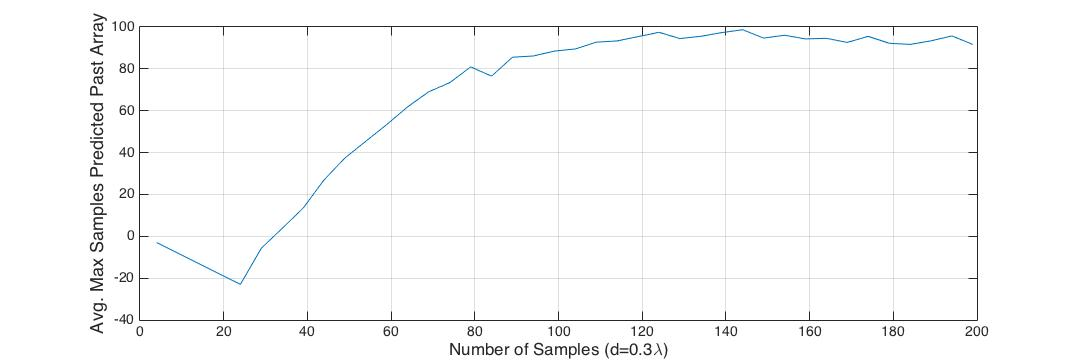
\includegraphics[width=\textwidth]{Small_N_1000}
\caption{AMPL vs. number of samples in sampling array for an example scenario with 7 scatterers with uniform probability distribution in angle, SNR = 15 dB, 100 snapshot averaging, sample spacing = $0.3 \lambda$, and equal scattering path amplitudes.}\label{sim_vs_samples}
\end{center}
\end{figure}
\begin{figure}
\begin{center}
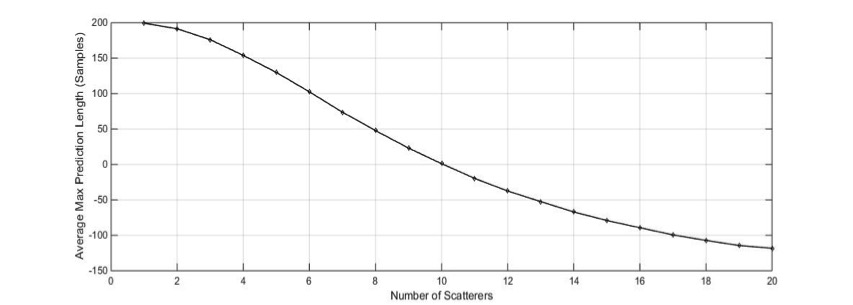
\includegraphics[width=\textwidth]{sim_vs_numScat}
\caption{AMPL vs. number of scatterers in environment for an example scenario with 133 samples in sampling array, SNR = 13 dB, 100 snapshot averaging, sample spacing = $0.3 \lambda$, and equal scattering path amplitudes.}\label{sim_vs_numScat}
\end{center}
\end{figure}
\begin{figure}
\begin{center}
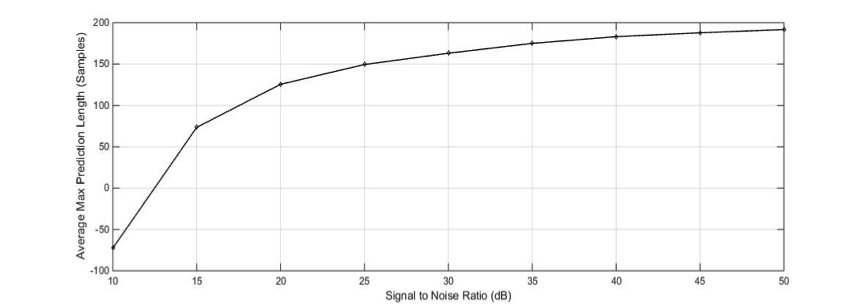
\includegraphics[width=\textwidth]{sim_vs_SNR}
\caption{AMPL vs. signal to noise ratio for an example scenario with 7 scatterers with uniform probability distribution in angle, 133 samples in sampling array, 100 snapshot averaging, sample spacing = $0.3 \lambda$, and equal scattering path amplitudes.}\label{sim_vs_SNR}
\end{center}
\end{figure}


\emph{Experiment summary and results go here}


\newpage
\subsection*{Technical Approach and Timeline}
This project's technical activities focus on four major avenues of research, which will be conducted in parallel: theoretical analysis of LSK security; investigation of generalized eavesdropping scenarios; experimental demonstration in realistic channels; and mitigation strategies for legitimate nodes.  Figure \ref{timeline} shows the timeline for these activities. 
\subsubsection*{Task 1: Theoretical Analysis of Link Signature Keying Security}
Theoretical analysis of LSK security will initially focus on the linear eavesdropper scenario that was used in the preliminary work discussed above, then generalize these results to alternative eavesdropping scenarios.  This task will analyze the relationship between the MSD and the parameters of the channel and eavesdropper array using techniques from information theory and estimation theory.  Specific activities include quantifying the information loss due to ``processing'' of the channel parameters to produce the legitimate and eavesdropper channel transfer functions, establishing a definition of the MSD that is based on an upper bound on the mutual information, and determining whether an MSD exists that does not depend on the eavesdropper array parameters.  It is expected that these results will depend on the assumed physical channel model and eavesdropper scenario, so these questions will be readdressed as additional scenarios are examined.
%I shouldn't say yet, because I haven't done it, but the way to derive the MSD is to find the capacity of some combination of channels where the things that get measured are \theta, h_E, h_B. This would mean the prob dist of theta that maximizes mutual information between some pair of these quantities, because that's what we use to find channel capacity.  
%Information theoretic argument to find MSD based on upper (not lower) bound on MI.  If we assume we don't know the prob dist of $\theta$, this amounts to finding the prob dist for $\theta$ that maximizes $I(h_{AE}, h_{AB})$, under some constraints (maybe we know the angular spread and other things about the channel).  Which, in turn, is kind of the capacity of a ``meta-channel.'' 

\subsubsection*{Task 2: Generalized Eavesdropping Scenarios}
This task will generalize the preliminary and theoretical analysis of the linear eavesdropper with far-field scatterers to additional scenarios.  These scenarios will eliminate some of the simplifying assumptions that were applied to the scenario in initial work.  The theoretical analysis produced in Task 1 for the linear case will be applied and generalized.  For instance, Eve may have only noisy estimates rather than perfect knowledge of any node's location; the scatterers may not be in the far field of the observation window, necessitating a time difference of arrival approach; Eve may have a single antenna that passes through a time-varying scene, which would invite the use of synthetic aperture radar techniques; or Eve's samples may be in some configuration other than a line, such as a grid, circle, or random distribution.  In each case, theoretical analysis and Monte Carlo simulation will be used to predict the eavesdropper's estimation capabilities, then relevant scenarios will be implemented in a software-defined radio testbed as described below.

%\begin{itemize}
%\item Eve doesn't have perfect knowledge of any node's location, just a noisy estimate
%\item Scatterers not in far field, so it's a TDOA problem
%\item Eve has a single antenna that passes through the scene, so it's a SAR problem
%\item Eve's samples are in some other configuration (grid, circle around B, random locations) rather than a line
%\item Eve's nodes are not coherent and have to be calibrated after measurement (but maybe locations are known?)
%\end{itemize}
\subsubsection*{Task 3: Software-Defined Radio Testbed for Link Signature Keying}
Tasks 1, 2, and 4 will be supported by implementation of a software-defined radio testbed for LSK experiments.  The testbed is implemented using Ettus USRP X310 radios, which support operating frequencies between 10 and 6000 MHz using UBX daughterboards and can be reprogrammed for a variety of test scenarios.  The testbed will include independent radios for Alice and Bob, and an eight-radio array (32 receive channels) for Eve, for a total of 10 USRP X310s.  The eavesdropping array will allow simultaneous multichannel recording in order to test eavesdropper strategies in mobile channels. Experiments will be conducted in an existing electromagnetically shielded room at UMB and in realistic indoor and outdoor environments.  The testbed will be used to implement a variety of channel scenarios  and verify the results of the first two tasks.  Most results on LSK implementations are implemented using WiFi systems, but the wide bandwidth and swappable daughterboards supported by the proposed testbed will permit future investigation of HF and UHF channels and, with LFRX/LFTX radio daughterboards and appropriate transceivers, even underwater ultrasound scenarios.
%Alice radio Tx/Rx
%Bob radio Tx/Rx
%Eve multiple radios - how many samples do we need? Let's say 20ish would be enough with half-wavelength spacing - CRLB predicts good estimation out to 8 wavelengths, but it's just the zero-crossing point in the simulation. Maybe 32 would be better.  Each radio supports 4 Rx channels (real samples only if used this way), which would mean 8 radios.
%total: 10 radios, 10 computers to supervise them, 20 UBX daughterboards.  If ultrasound, 18 LFRX and 2 LFTX daughterboards. Total: 50k + 20k + 22k = 92k
%plus more for LFRX/LFTX and ultrasound transceivers (could get letter of collab from Tommaso)

%\begin{itemize}
%\item Development of software-defined radio testbed
%\item Alternative channels (most results are wifi) - HF (ionosphere), underwater, indoor/outdoor differences, UHF
%\item Simultaneous multichannel recording, which is needed for mobile channels %can an SDR system do this?  Maybe with many radios, processing on FPGA, and Ettus's "MIMO" features - or with a more sophisticated less hacky system - examine options
%\item testing a variety of eavesdropper configurations
%\end{itemize}
\subsubsection*{Task 4: Mitigation Strategies for Legitimate Nodes}
The tasks discussed above have primarily focused on characterizing the capabilities of an eavesdropper in an LSK scenario.  However, the goal of these efforts is to realize quantifiably secure and practical LSK systems, which necessarily involves examining the behavior of the legitimate nodes as well.  Toward that goal, the last major research task of this project will investigate mitigation strategies for legitimate nodes to use against a known or suspected eavesdropper.  These may include manipulating of the channel itself or the legitimate nodes' antennas to improve the security achievable via LSK \cite{chen2011, mehmood2015}; identifying whether a channel is suitable or unsuitable for LSK; estimating the minimum secure distance from channel observations; and adapting the key generation protocol in response to channel or eavesdropper properties (if known).  This portion of the project applies the results of the other research tasks to provide concrete recommendations, based on our new minimum secure distance paradigm, for implementation of LSK systems in the presence of potentially sophisticated eavesdroppers.

%\begin{itemize}
%	\item channel manipulation/antenna features \cite{chen2011, mehmood2015}
%	\item selecting (or creating!) a hospitable channel
%	\item changes to network protocol 
%\end{itemize}
\begin{figure}
\begin{center}
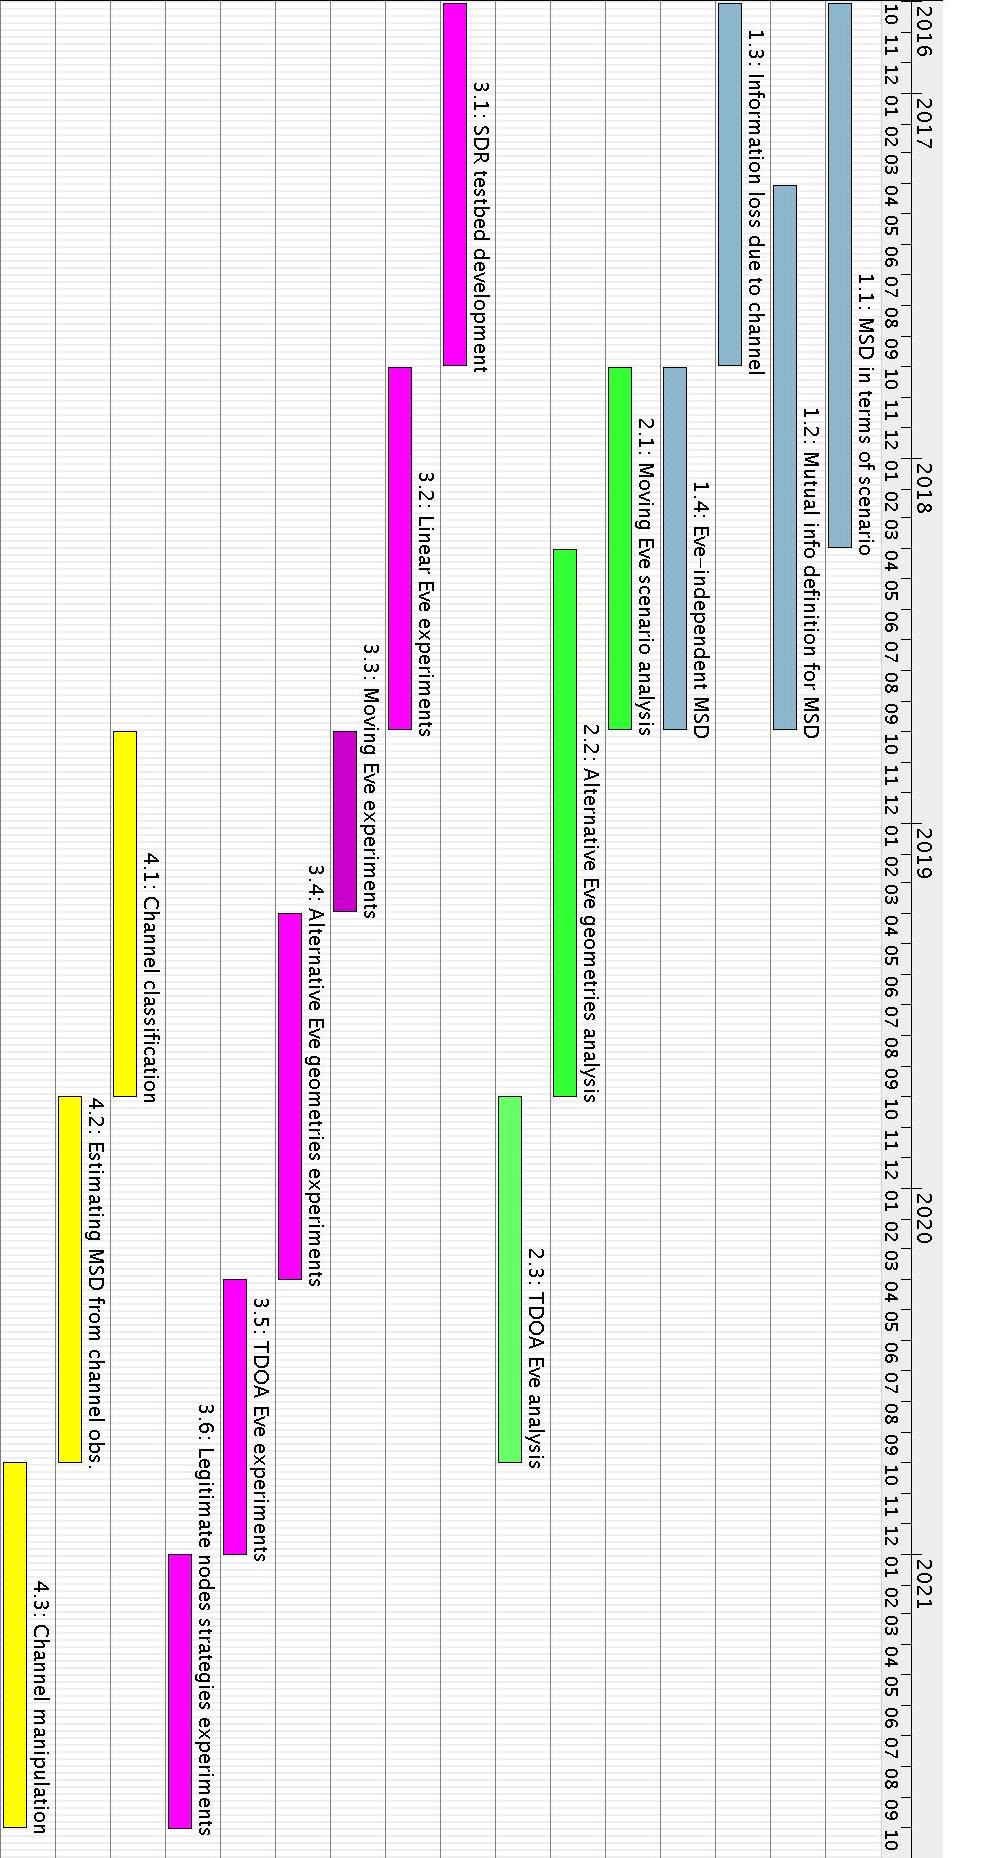
\includegraphics[height=0.95\textheight]{NSF_proj_gantt.jpg}
\caption{Timeline of technical activities.  Task 1 is blue, Task 2 green, Task 3 magenta, Task 4 yellow.}\label{timeline}
\end{center}
\end{figure}
\clearpage

\subsection*{Risks}
\subsubsection*{Schedule Risk}
In a long-term project, dependencies between tasks can cause delays if early tasks take longer than expected.  The project plan avoids this common issue by ensuring that tasks are independent wherever possible.  For instance, the experimental work in Task 3 is informed by theoretical results from Tasks 1, 2, and 4 if they are available, but does not depend on those results for completion.  Similarly, Tasks 2 and 4 require similar background information and analysis techniques to Task 1, but are independent of its results.  

\subsubsection*{Technical Risk}
Technical risks are also a concern in any research project.  Theoretical tasks like Tasks 1, 2, and 4 face the risk that a proposed method cannot be used to achieve the desired result.  The proposed approach mitigates this risk by including multiple alternative techniques  -- for instance, an information theoretic approach, an estimation theoretic approach, and simulation.  If all the techniques are effective, the comparable results will validate and reinforce one another.  If one approach fails, the other avenues of research ensure that the project itself does not.

Experimental tasks include the risk of unanticipated setbacks during implementation. This proposal mitigates that risk by allocating sufficient development time to the testbed; and proposing a variety of experiments that can be conducted using the same hardware and control software, which minimizes additional development work required between tests.

\subsubsection*{Staffing and Training Risk} %refer to educational plan
Working with students always presents a degree of risk: they must develop skills and become familiar with a new field while making tangible progress on the project.  This risk can be mitigated by having a well-defined training sequence, and is addressed here by the first part of the education plan.  No course in wireless or digital communications is currently offered at UMass Boston, so the course serves as both a training and recruiting tool.  Selected modules from the course can also be used asynchronously by students who need an introduction to particular topics.

%CS grad student would have nice coding and may have been exposed to sigproc in the context of computer vision - how to make this an interesting problem in CS (computer vision/big data/machine learning)?  ask a CS prof for suggestions/to co-advise.
\subsection*{Evaluation}
\begin{itemize}
	\item What conditions ensure arbitrarily low mutual information between Eve and Alice/Bob?
	\item How does the security of our proposed system compare to that of one using correlation length as secure distance?  (Use MI if possible to characterize this)
	\item How well does channel reconstruction eavesdropping work in realistic channels? - evaluation of theoretical work \& results is also supported by experimentation using SDR testbed
	\item Can Alice and Bob manipulate the LSK scenario to improve their security?
	\item publications - particularly crucial each task is expected to produce multiple
\end{itemize}
\subsection*{Future Work}
\begin{itemize}
\item Most LSK results use WiFi, and this proposal focuses on the non line of sight rayleigh fading environments that are typical of WiFi channels. 
\item Extend theoretical results to other types of channels (Rician, etc.); 
\item use flexibility of testbed to test at HF, UHF frequencies and in underwater scenarios
\item propose statistical channel models that are more suitable for LSK (i.e. don't always assume Gaussian statistics)
\item Examine effects of shadowing, non-point scatterers, etc.
\end{itemize}

\section*{Education Plan}
\subsection*{Generating Interest in Wireless Communications Research via Undergraduate Education}
%hard to get students interested in wireless comms because its emag and sigproc aspects are perceived as "hard"
%Comms is often a graduate level course
%make it accessible to undergrads using USRP examples
%generate interest in research by introducing current comms problems (not just CREW but also...)
%involve students in experiment implementation!

%text: J.G. Proakis and M. Salehi, Fundamentals of Communication Systems

%Outline:
	%review of sigproc concepts, special attention to digital
		%DFT lab: relationship between sampling rate & FFT bandwidth, FFT length & resolution.
	%analog to digital conversion
		%encoding
		%pulse code modulation
		%phase modulation (BPSK, QPSK) and eye diagrams lab activity
	%probability and random processes; noise
		%lab activity on signal to noise ratio effect on eye diagram and bit error rate
	%OFDM
		%lab activity - implement OFDM system
		%research highlight - why equalization, pre-distortion, and channel prediction are important & interesting
	%wireless channels and multipath
		%lab activity - ISI, delay spread, etc. and effect on OFDM system
		%lab activity/research highlight - LSK experiment implementation example
		%research highlight - MIMO
	


\subsection*{Grad Launchpad}
%UMB serves most diverse student population in new england
%In UMB's first graduating class, one student (out of 11) enrolled in graduate school - aim is to increase that percentage as department and enrollment grow
%Inclusive program to help underrepresented students navigate pathways to grad education: seminars, workshops, and panel discussions for CSM students
	% Students might not be aware of advantages - talk about average salaries, differences in work responsibilities, etc.
	% Students may not know how to pay for it ("Diversity & inclusiveness" report)
	% Even if they want to do grad school, they may need help navigating the application process
	% Support development of graduate school skills - networking, communication, writing a CV, etc.
	
%Grad Launchpad 0: viral sticker campaign, "grad launchpad" website

%Grad Launchpad 1: "Is grad school worth it/how will I pay for it?" seminar - Sept/Oct
%Grad Launchpad 2: "Applying - and getting in" workshop - Oct/Nov 
%Grad Launchpad 3: "What is grad school like?" panel - Nov/Dec

%Grad Launchpad 5: "Applying - and getting in" workshop #2 - Feb/Mar 
%Grad Launchpad 6: "What is it good for?" jobs panel - Mar/Apr
%Grad Launchpad 7: "Skills for grad school" workshop - Apr/May  - how to read a paper, professional communication, writing a CV

\subsection*{Evaluation}
%evaluate course using pre- and post- surveys on exposure to and interest in wireless comms
%evaluate grad launchpad program using class-wide pre- and post- surveys on interest in and confidence about getting a grad degree, and the number of students each year who apply to grad school and enroll


\section*{Broader Impacts}  
%impact of both ed plan and research plan, and how they are related to each other.
\bibliography{PL-Library}
\end{document}